\documentclass{beamer}
\usetheme{Frankfurt}
\usepackage{fontspec}
\usepackage{graphicx}
\usepackage{tikz}
\usepackage[english,russian]{babel}
\usepackage{xltxtra}
\usepackage{xunicode}
\setbeamertemplate{navigation symbols}{}
\setbeamertemplate{footline}{}
\defaultfontfeatures{Scale=MatchLowercase,Mapping=tex-text}
\begin{document}
\newcommand{\fn}{\fontspec{Arial}}
\fn
\setbeamerfont{listfn}{size=\Large}
\setbeamerfont{resetfn}{size=\normalsize}
\title{\fontsize{20pt}{22pt}\fn\selectfont
Система обліку платних курсів із підтримкою самостійного запису слухачів через мережу Інтернет. Підтема 1. Модуль обліку платних курсів
}
\author{\fontsize{24pt}{26pt}\fn\selectfont
Студент --- Горбешко Б. М.\\Керівник --- Оніщенко Т. В.
}
\date{}
\frame{\titlepage}
\begin{frame}{\fn Причина і мета розробки}

{\fontsize{14pt}{16pt}\fn\selectfont
\parbox{11cm}{
Причиною розробки автоматизованої системи обліку платних курсів є відсутність такої системи на кафедрі Системного програмного забезпечення.
}
\\[\baselineskip]
\parbox{11cm}{
Метою створення системи є зменшення часу, що витрачається працівниками кафедри на пов'язану з курсами роботу шляхом автоматизації набору слухачів на курси, реєстрацій сплат та формування звітності, а також для надання майбутнім слухачам можливості ознайомитися з наявними курсами та залишати заявки на реєстрацію за допомогою зовнішніх програмних сервісів.
}
}
\end{frame}
\begin{frame}{\fn Діаграма концептуальних класів}
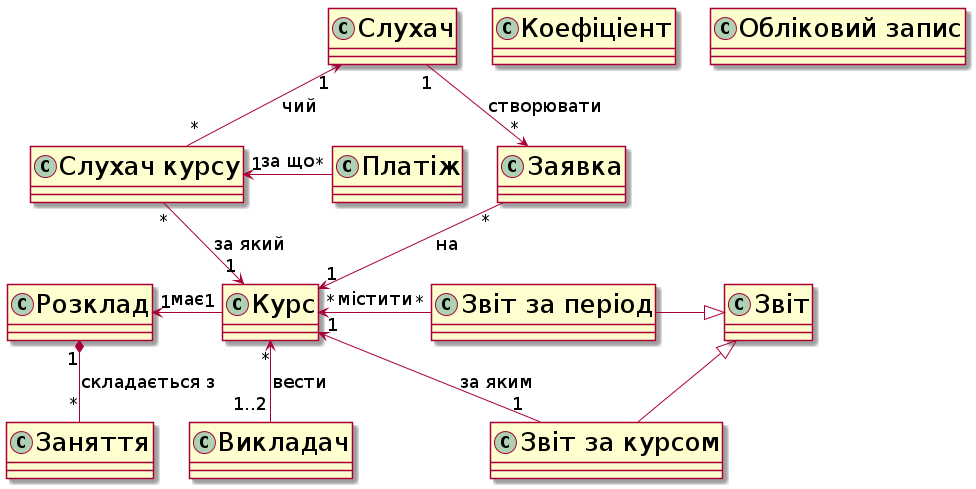
\includegraphics[width=11cm]{pp_pw3_conc_pres.png}
\end{frame}
\setbeamertemplate{itemize/enumerate body begin}{\fontsize{18pt}{20pt}\fn\selectfont}
\begin{frame}{\fn Вимоги}
\begin{itemize}
\item Робота з слухачами, курсами, викладачами, розкладом, сплатами за курси
\item Відображення та редагування даних у таблицях
\item Формування придатних до друку звітів
\item Web-інтерфейс
\item Вкладені таблиці для сутностей M--M
\end{itemize}
\end{frame}
\setbeamertemplate{itemize/enumerate body begin}{\fontsize{24pt}{26pt}\fn\selectfont}
\begin{frame}{\fn Аналогічні системи}
\begin{itemize}
\item 1C: Бухгалтерія
\item Парус
\item 1C-Бітрікс: Внутрішній портал навчального закладу
\item Moodle
\item Веб-застосунок MS Access + SharePoint
\end{itemize}
\end{frame}
\begin{frame}{\fn Діаграма прецедентів}
\vspace{0cm}
\begin{center}
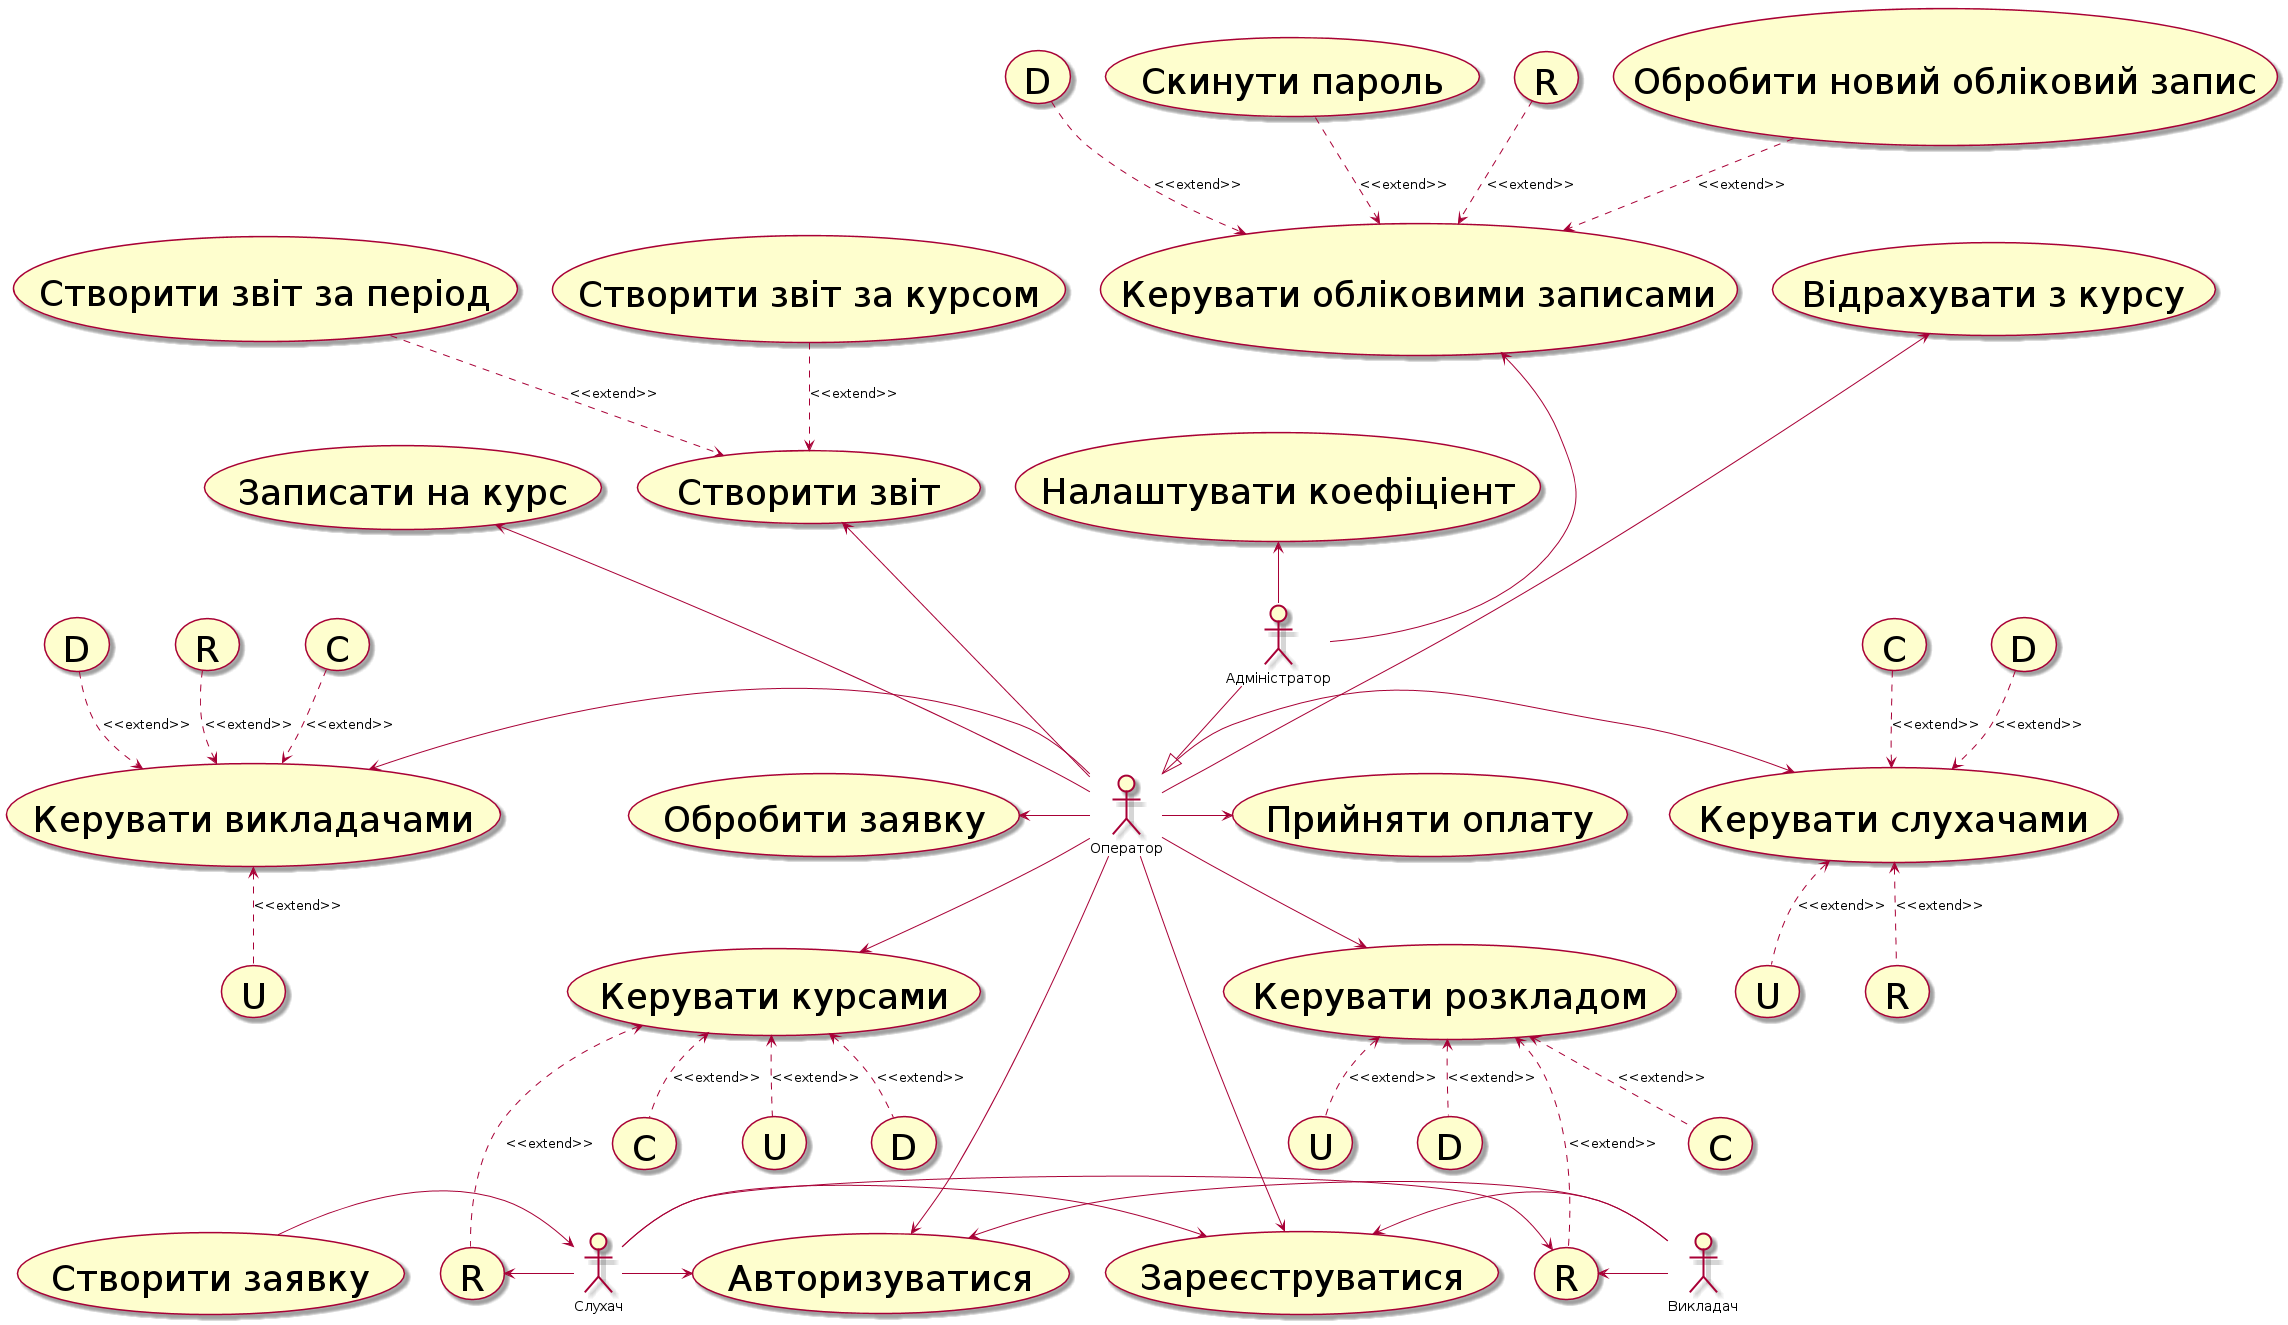
\includegraphics[width=11cm]{pp_pw1_uc_pres.png}
\end{center}
\end{frame}
\begin{frame}{\fn Діаграма програмних класів}
\begin{center}
\vspace{-3mm}
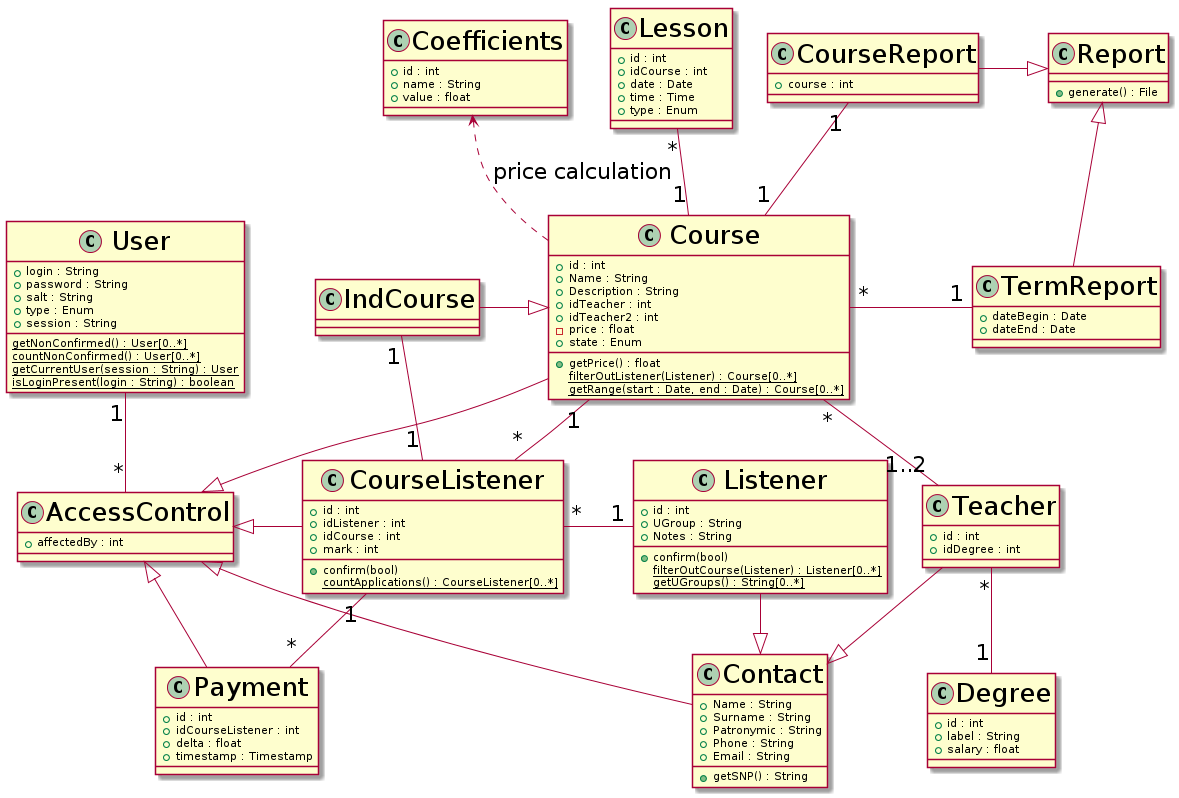
\includegraphics[width=11cm]{pp_pw3_clas_pres.png}
\end{center}
\end{frame}
\begin{frame}{\fn Схема бази даних}
\begin{center}
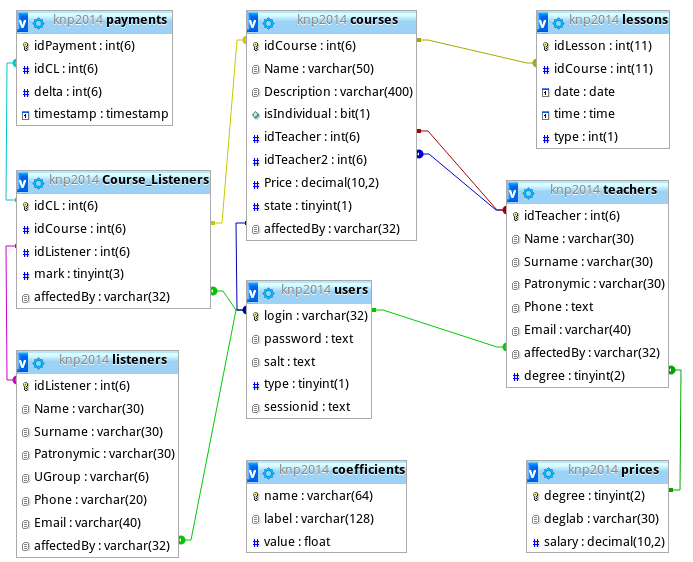
\includegraphics[width=8cm]{scrns/db.png}
\end{center}
\end{frame}
\begin{frame}{\fn Архітектура програмних модулів}
\begin{itemize}
\item entities
 \begin{itemize}
 \item coefficient
 \item course
 \item courses\_of\_listener
 \item ind\_course
 \item lesson
 \item listener
  \begin{itemize}
  \item check.php
  \item create.php
  \item read.php
  \item update.php
  \item destroy.php
  \item \ [rel.php]
  \item dataSource.json
  \item scheme.json
  \end{itemize}
 \item listeners\_of\_course
 \item payment
 \item price
 \item teachers
 \end{itemize}
\end{itemize}
\end{frame}
\begin{frame}{\fn Головне меню системи}
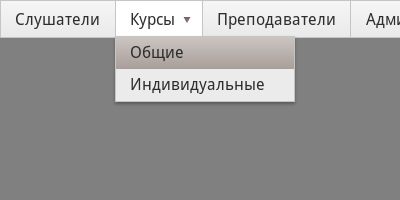
\includegraphics[width=5cm]{scrns/menu1.png}\quad
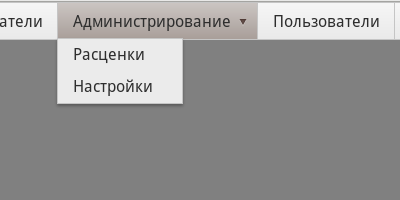
\includegraphics[width=5cm]{scrns/menu2.png}
\begin{center}
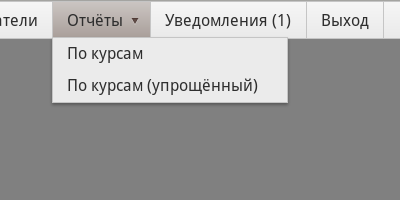
\includegraphics[width=5cm]{scrns/menu3.png}
\end{center}
\end{frame}
\begin{frame}{\fn Приклад таблиці}
\begin{center}
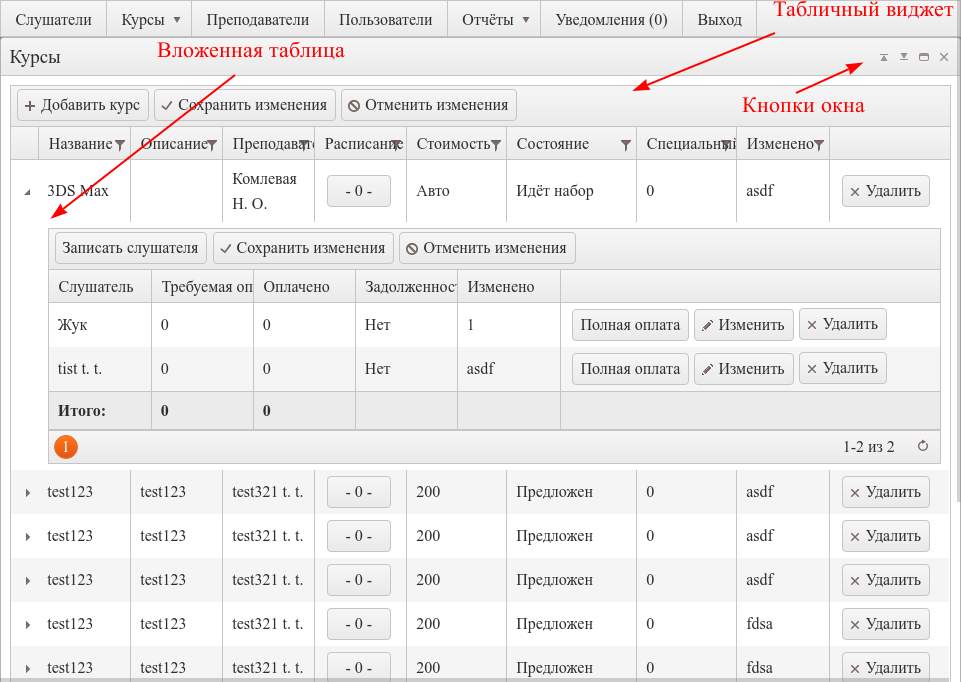
\includegraphics[width=10cm]{scrns/scrn3.png}
\end{center}
\end{frame}
\begin{frame}{\fn Сповіщення}
\begin{center}
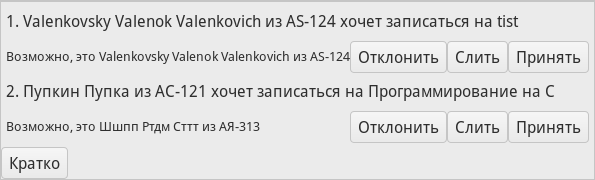
\includegraphics[width=10cm]{scrns/notifications1.png}\\
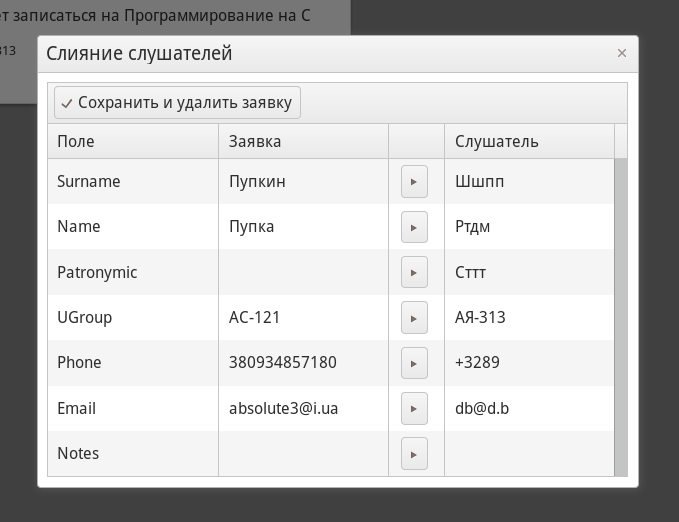
\includegraphics[width=6cm]{scrns/notifications2.png}
\end{center}
\end{frame}
\begin{frame}{\fn Звіт}
\begin{center}
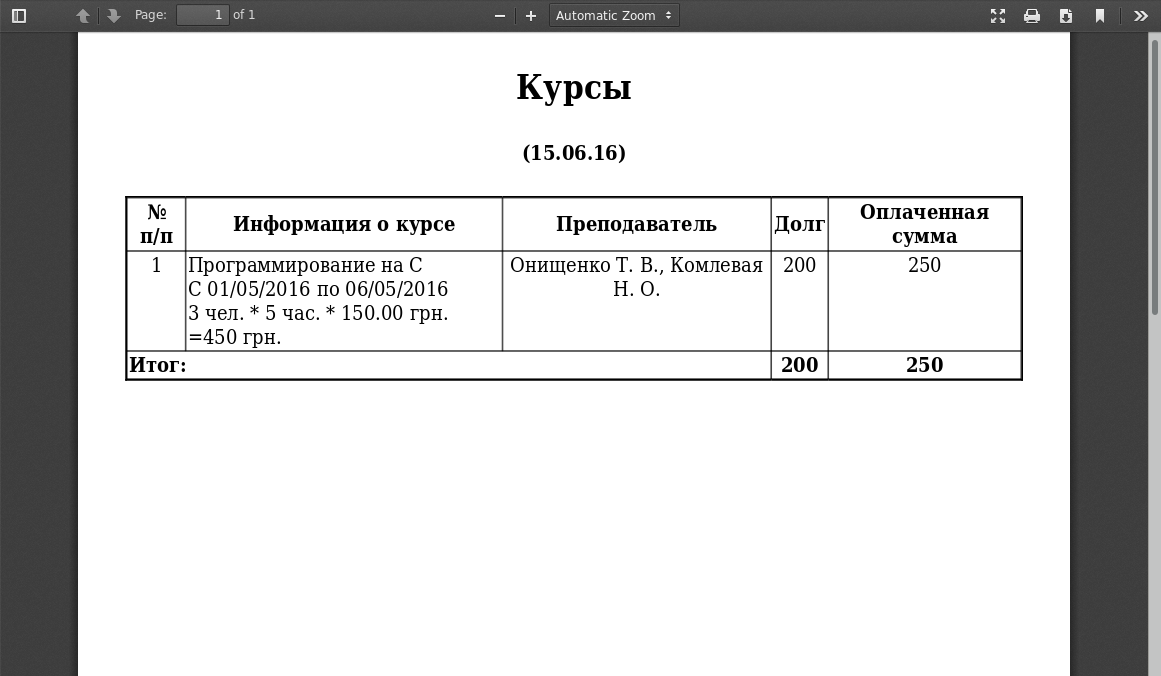
\includegraphics[width=11cm]{scrns/report.png}
\end{center}
\end{frame}
\begin{frame}{}
\begin{center}
{\fontsize{48pt}{48pt}\selectfont Дякую за увагу!}
\end{center}
\end{frame}
\end{document}
